\documentclass{article}

\usepackage{PRIMEarxiv}

\usepackage[utf8]{inputenc}
\usepackage[T1]{fontenc}
\usepackage[colorlinks=true,allcolors=blue]{hyperref}
\usepackage{url}
\usepackage{booktabs}
\usepackage{amsfonts}
\usepackage{amsmath}
\usepackage{amssymb}
\usepackage{amsthm}
\usepackage{nicefrac}
\usepackage{microtype}
\usepackage{fancyhdr}
\usepackage{graphicx}
\graphicspath{{media/}}
\usepackage[numbers]{natbib}
\usepackage{algorithm}
\usepackage{algpseudocode}
\usepackage{tikz}
\usetikzlibrary{arrows.meta,positioning,fit}

\newtheorem{definition}{Definition}
\newtheorem{proposition}{Proposition}

\newcommand{\R}{\mathbb{R}}
\newcommand{\E}{\mathbb{E}}
\newcommand{\T}{\mathcal{T}}
\newcommand{\G}{\mathcal{G}}
\newcommand{\Vset}{\mathcal{V}}
\newcommand{\Eset}{\mathcal{E}}
\newcommand{\In}{\mathcal{I}}
\newcommand{\Out}{\mathcal{O}}
\newcommand{\sg}{\operatorname{sg}}
\newcommand{\clip}{\operatorname{clip}}
\newcommand{\expl}{\ell}

% Header
\pagestyle{fancy}
\thispagestyle{empty}
\rhead{\textit{CS329 Project Idea Review}}
\fancyhead[LO]{Learning to give up with a fly's give-up circuit}

\title{Can a Fly's Give-Up Circuit Learn to Give Up?\\
Multi-Agent Reinforcement Learning in the War of Attrition with Connectome-Wired Policies
\thanks{\textit{\underline{Project idea review}}: CS329 Foundations of AI: Multi-Agent Systems, IIT Gandhinagar, 2026.}}

\author{
  Suhani \\
  IIT Gandhinagar \\
  \texttt{suhani.24110358@iitgn.ac.in} \\
  \And
  Mayank Choudhary \\
  IIT Gandhinagar \\
  \texttt{mayank.choudhary@iitgn.ac.in} \\
  \AND
  Krina Paghadar \\
  IIT Gandhinagar \\
  \texttt{krina.paghadar@iitgn.ac.in} \\
  \And
  Nakshatra Lad \\
  IIT Gandhinagar \\
  \texttt{nakshatra.lad@iitgn.ac.in} \\
}

\begin{document}
\maketitle

\begin{abstract}
When two male fruit flies fight, one of them eventually gives up. The time at which it does so follows the exponential law that game theory predicts for the war of attrition, and recent work has traced this decision to a small circuit in the fly brain. The complete wiring diagram of the male fly nervous system now lets us copy that circuit neuron by neuron. We propose to turn the real give-up circuit into the policy network of a learning agent, let two such agents play the war of attrition against each other with reinforcement learning, and check whether the fly's wiring helps them find the equilibrium better or faster than networks of the same size with different wiring. This report sets up the game, explains how a circuit taken from the connectome becomes a trainable policy and how reinforcement learning updates it, and lists the comparisons, metrics and results we plan to show in the final submission.
\end{abstract}

\keywords{multi-agent reinforcement learning \and war of attrition \and connectome \and Drosophila \and self-play \and exploitability}

% ==================================================================
\section{Introduction}
\label{sec:intro}

Picture two animals fighting over food, where neither can really hurt the other and the only question is who keeps going longer. Waiting costs energy, and whoever stays longest gets the food. In 1974 John Maynard Smith showed that in this game, the war of attrition, no fixed waiting time can be a good strategy \citep{maynardsmith1974}. If you always wait exactly $t$ seconds, a rival who waits a little longer beats you every time. The only stable strategy is to wait a random amount of time, drawn from an exponential distribution whose average is the value of the food divided by the cost of waiting \citep{maynardsmith1974, bishop1978}. For fifty years this was a prediction about behaviour, with nothing to say about how a brain could produce such a random but well-calibrated decision.

That is now changing. \citet{ventimiglia2026} found that fighting male fruit flies really do give up at exponentially distributed times, and that the rate shifts with hunger and with the presence of food, exactly as it should if flies value the prize more when they need it more. They also found the circuit behind the decision. PPL1 dopamine neurons carry the ``this is going badly'' signal, two mushroom-body output neurons (MBON-18 and MBON-19) combine it, and giving up shows up as a long-lasting shutdown of the Tk-GAL4$^{\mathrm{FruM}}$ aggression neurons. At the same time, complete wiring diagrams (connectomes) of the fly brain have become available: the hemibrain \citep{scheffer2020}, FlyWire for the female brain \citep{dorkenwald2024}, and now MaleCNS for the whole male nervous system \citep{berg2026}. So for the first time we can take the exact wiring of a circuit that carries out a game-theoretic strategy and ask what that wiring is good for.

Researchers have already used fly connectomes as neural network architectures. \citet{lappalainen2024} built networks wired like the fly visual system and found that the wiring alone predicts how real neurons respond. \citet{jin2026} turned the whole fly brain into a graph neural network with fixed synapse weights and trained it with reinforcement learning to make a simulated fly body walk and fly \citep{vaxenburg2025}. Both treat the connectome as the controller of a single agent. Our setting is different because the war of attrition is a game between two agents. Its solution is a mixed equilibrium, not a single best action, and learning a mixed equilibrium through self-play is known to be tricky \citep{fudenberg1998, hofbauer2009}.

Our question is this. If two learning agents play the war of attrition, and each agent's policy network is wired exactly like the real fly give-up circuit, do they learn the equilibrium better or faster than agents whose networks have the same size but different wiring?

Two things make this question clean to answer. First, the equilibrium of the game is known exactly, so we can measure how far a learned strategy is from it without any approximation, using the exploitability measure of \citet{bichler2021}. Second, we can build exact controls. A degree-preserving rewire \citep{maslov2002} keeps how many connections each neuron has but shuffles who connects to whom, so any difference between the real circuit and its rewire comes from the specific wiring and nothing else. Either answer is useful. If the real wiring helps, the circuit may be shaped to learn this particular game well. If it does not, the circuit's role likely lies somewhere other than its wiring, for example in its chemistry, its timing, or the signals it receives.

% ==================================================================
\section{Preliminaries}
\label{sec:prelim}

\subsection{Games and equilibria}

A two-player game is $\Gamma = (N, (S_i)_{i\in N}, (u_i)_{i \in N})$ with players $N = \{1,2\}$, action sets $S_i$ and payoffs $u_i : S_1 \times S_2 \to \R$. It is symmetric if $S_1 = S_2 = S$ and $u_1(s,s') = u_2(s',s)$. In that case we write $u(s,s')$ for the payoff of playing $s$ against $s'$.

A mixed strategy is a probability distribution $\pi \in \Delta(S)$ over actions. Payoffs extend to mixed strategies by taking expectations, $u(\pi,\pi') = \E_{s \sim \pi,\, s' \sim \pi'}[u(s,s')]$. The support of $\pi$ is $\operatorname{supp}(\pi) = \{s : \pi(s) > 0\}$.

\begin{definition}[Symmetric Nash equilibrium]
$\pi^*$ is a symmetric Nash equilibrium if $u(\pi^*,\pi^*) \ge u(\pi,\pi^*)$ for every $\pi \in \Delta(S)$. Equivalently, every action in $\operatorname{supp}(\pi^*)$ earns the same payoff against $\pi^*$, and no action outside the support earns more.
\end{definition}

\begin{definition}[Evolutionarily stable strategy, ESS]
$\pi^*$ is an ESS if for every $\pi \ne \pi^*$, either $u(\pi^*,\pi^*) > u(\pi,\pi^*)$, or $u(\pi^*,\pi^*) = u(\pi,\pi^*)$ and $u(\pi^*,\pi) > u(\pi,\pi)$ \citep{maynardsmith1974}.
\end{definition}

\begin{definition}[Stable game]
A symmetric game with a finite action set and payoff matrix $U$ is strictly stable if $z^\top U z < 0$ for every nonzero $z$ with $\mathbf 1^\top z = 0$. Such a game has exactly one symmetric equilibrium, and standard learning dynamics converge to it \citep{hofbauer2009}.
\end{definition}

\subsection{Distance from equilibrium}

\begin{definition}[Exploitability]
The exploitability (ex-ante utility loss) of a strategy $\pi$ against an opponent strategy $\pi'$ is
\[
\expl(\pi;\pi') = \max_{s\in S} u(s,\pi') - u(\pi,\pi').
\]
It is how much a player using $\pi$ could gain by switching to the best response. $\pi^*$ is a symmetric equilibrium exactly when $\expl(\pi^*;\pi^*) = 0$ \citep{bichler2021}.
\end{definition}

\subsection{Policies and policy-gradient learning}

A policy $\pi_\theta(s \mid x)$ is a probability distribution over actions produced by a network with parameters $\theta$ from an input (context) $x$. Given sampled actions $s_j$ with payoffs $u_j$ and a baseline $\bar u$ (the average payoff so far), the REINFORCE gradient estimate \citep{williams1992} is
\[
\hat g = \frac1B \sum_{j=1}^{B} (u_j - \bar u)\, \nabla_\theta \log \pi_\theta(s_j \mid x).
\]
The quantity $A_j = u_j - \bar u$ is called the advantage. Actions that did better than usual become more likely, and actions that did worse become less likely.

Proximal policy optimisation (PPO) \citep{schulman2017} reuses one batch of experience for several updates. It measures how much the policy has moved using the ratio $r_j(\theta) = \pi_\theta(s_j\mid x)/\pi_{\theta_{\mathrm{old}}}(s_j \mid x)$ and maximises
\[
L^{\mathrm{clip}}(\theta) = \frac1B \sum_j \min\!\Big( r_j(\theta) A_j,\; \clip\big(r_j(\theta), 1-\epsilon, 1+\epsilon\big) A_j\Big),
\]
which stops the policy from moving too far from the one that collected the data.

\subsection{Connectomes as graphs}

A connectome is a directed graph $\G = (\Vset, \Eset, w)$. Its vertices are neurons, an edge $(j \to i)$ means neuron $j$ makes synapses onto neuron $i$, and $w_{ij} \in \mathbb N$ is the number of those synapses. Each neuron also has a predicted neurotransmitter \citep{eckstein2024}. Under Dale's principle this fixes the sign $\sigma_j \in \{+1,-1,0\}$ of all of neuron $j$'s outgoing connections: $+1$ for excitatory, $-1$ for inhibitory, and $0$ for modulatory or unknown. For a set of neurons $\Vset'$, $\G[\Vset']$ is the subgraph containing only those neurons and the edges between them. The in-degree $d^{\mathrm{in}}_i$ and out-degree $d^{\mathrm{out}}_i$ count the incoming and outgoing edges of neuron $i$.

A degree-preserving rewire \citep{maslov2002} repeatedly picks two edges $(a \to b)$ and $(c \to d)$ and swaps them to $(a\to d)$ and $(c \to b)$, skipping swaps that would create self-loops or duplicate edges. Every neuron keeps its in- and out-degree, and everything else about the wiring is randomised.

% ==================================================================
\section{Problem Formulation}
\label{sec:formulation}

\subsection{The problem}

Two agents repeatedly play the war of attrition. In each round, each agent picks how long to stay in the fight. Each agent's strategy comes from a neural network, and the network is wired exactly like the fly's give-up circuit: neurons from the connectome become units, and synapses become connections. The agents improve their strategies over many rounds using reinforcement learning, only from the payoffs they experience. We know exactly what the equilibrium strategy is, so we can track how close the agents get to it and how fast. We then repeat everything with networks of the same size whose wiring is not the fly's. The problem is to find out whether the real wiring makes any difference to how well and how fast the agents learn the equilibrium.

\subsection{The game}

Let $V > 0$ be the value of the prize and $c > 0$ the cost of fighting per unit time. Each player picks a quitting time $t \ge 0$. Both pay $c \min(t,t')$, and the one who stays longer wins $V$:
\[
u(t,t') =
\begin{cases}
V - c\,t' & t > t',\\
-c\,t & t < t',\\
V/2 - c\,t & t = t'.
\end{cases}
\]

\begin{proposition}[\citealp{maynardsmith1974, bishop1978}]
The game has a unique symmetric equilibrium, which is also its ESS: $T \sim \mathrm{Exp}(c/V)$, so $P(T > t) = e^{-ct/V}$ and $\E[T] = V/c$. The equilibrium payoff is $0$.
\end{proposition}

We use $V = c = 1$, so the equilibrium is $T \sim \mathrm{Exp}(1)$. Time is placed on a grid $\T = \{t_k = k\Delta\}_{k=0}^{n-1}$ with $n = 64$ points, $T_{\max} = 8$ and $\Delta = T_{\max}/(n-1)$. On the grid the game becomes a $64 \times 64$ matrix game $U = V\,W + C$, with $W_{kl} = \mathbb 1[k>l] + \tfrac12 \mathbb 1[k=l]$ and $C_{kl} = -c\min(t_k,t_l)$. This grid game is strictly stable, so it has one symmetric equilibrium $p^*$. It is geometric, $p^*_k \propto r^k$ with $r = \sqrt{1+(c\Delta/V)^2} - c\Delta/V$, and matches the exponential rounded down onto the grid.

\subsection{The circuit}

Let $\G^\star = (\Vset^\star, \Eset^\star, w, \sigma)$ be the MaleCNS v1.0 connectome \citep{berg2026}, keeping only edges with $w_{ij} \ge 5$ synapses. The three core cell populations from \citet{ventimiglia2026} are
\[
P = \{\text{PPL101--PPL108}\}\ (16\ \text{neurons}),\qquad
M = \{\text{MBON18, MBON19}\}\ (6),\qquad
Q = \{\text{AVLP727m}\}\ (5),
\]
where AVLP727m is the MaleCNS name for the Tk-GAL4$^{\mathrm{FruM}}$ neurons. Let $X$ be every neuron on a directed path of at most 3 synapses from $M$ to $Q$, and let $Y$ be every neuron that exchanges at least 400 synapses with $P \cup M \cup Q \cup X$. The circuit is
\[
\G = \G^\star[P \cup M \cup Q \cup X \cup Y], \qquad |\Vset| = 258,\ |\Eset| = 4{,}952.
\]
The input neurons are $\In = P$ and the output neurons are $\Out = Q$.

\subsection{Agents and controls}

For any graph $\G'$ on the same neurons, let $\Pi(\G')$ be the set of policies $\pi_\theta(\cdot \mid x) \in \Delta(\T)$ computed by a recurrent network whose connections are exactly the edges of $\G'$ (Section~\ref{sec:method} gives the exact form). We compare the real circuit $\G$ against:
\begin{itemize}
  \item $\mathcal D_{\mathrm{rew}}(\G)$, random degree-preserving rewires of $\G$;
  \item $\mathcal D_{\mathrm{rand}}(\G)$, random graphs on $\Vset$ with the same number of edges;
  \item a dense network $\Pi_{\mathrm{MLP}}$ (two hidden layers) with about the same number of trainable parameters.
\end{itemize}
All circuit-based networks keep the same neurons, the same input and output neurons, and the same neuron signs, so they have exactly the same number of parameters.

\subsection{The research question}

Let $\theta_\tau$ be an agent's parameters after $\tau$ rounds of learning, and $\expl_\tau$ its exploitability. Let $\tau_\varepsilon = \min\{\tau : \expl_\tau \le \varepsilon\}$ be the first round at which exploitability falls below $\varepsilon$. For a learning rule $\mathcal L$ and training length $T$, we want to estimate
\[
\delta_{\mathrm{rew}} = \E\big[\expl_T(\Pi(\G))\big] - \E_{\G' \sim \mathcal D_{\mathrm{rew}}(\G)}\big[\expl_T(\Pi(\G'))\big],
\qquad
\delta_{\mathrm{rand}} = \E\big[\expl_T(\Pi(\G))\big] - \E_{\G' \sim \mathcal D_{\mathrm{rand}}(\G)}\big[\expl_T(\Pi(\G'))\big],
\]
and the same differences for $\tau_\varepsilon$, and test whether they are zero. $\delta_{\mathrm{rew}}$ measures the effect of the fly's specific wiring. $\delta_{\mathrm{rand}} - \delta_{\mathrm{rew}}$ measures the effect of the degree pattern. Comparing $\Pi(\G')$ with $\Pi_{\mathrm{MLP}}$ measures the effect of using a sparse recurrent circuit at all.

% ==================================================================
\section{Methodology: How the Fly Circuit Learns}
\label{sec:method}

This section explains, step by step, how a piece of the fly connectome becomes an agent that plays the game and improves through reinforcement learning. Figure~\ref{fig:loop} shows the whole loop and Algorithm~\ref{alg:train} gives it as pseudocode.

\subsection{Step 1: from connectome to network}

Every one of the 258 neurons in $\G$ becomes one unit in a recurrent network, with an activity value $h_i$. Every one of the 4{,}952 edges becomes one trainable weight $\theta_{ij}$. Put these in a matrix $A_\theta$ with $(A_\theta)_{ij} = \theta_{ij}$ if $(j \to i) \in \Eset$, and $0$ otherwise. The zeros are fixed: the network can never create a connection that the fly does not have. At the start of training the weights are random, with scale $1/\sqrt{d^{\mathrm{in}}_i}$.

In the sign-constrained version we also respect Dale's principle. For a neuron with $\sigma_j \ne 0$ we write $\theta_{ij} = \sigma_j\, \mathrm{softplus}(\tilde\theta_{ij})$ and train $\tilde\theta_{ij}$ instead, so an excitatory neuron's outgoing weights stay positive and an inhibitory neuron's stay negative throughout learning.

\subsection{Step 2: one forward pass (the fly ``thinks'')}

The game context $x = V/c$ enters the circuit only through the 16 PPL1 input neurons. The signal then spreads through the wiring for $L = 6$ steps:
\[
h^{(0)} = 0,\qquad
h^{(\ell+1)} = \tanh\!\big(A_\theta h^{(\ell)} + E_{\In} W_{\mathrm{in}} x + b\big), \quad \ell = 0,\dots,L-1.
\]
Here $E_{\In}$ places the input on the PPL1 neurons, $W_{\mathrm{in}} \in \R^{16}$ is the input weight of each PPL1 neuron, and $b \in \R^{258}$ is a bias per neuron. At each step a neuron adds up the activity of the neurons that synapse onto it, weighted by $\theta_{ij}$, and passes it through $\tanh$. We use $L = 6$ because the core path PPL1 $\to$ MBON $\to$ two connecting neurons $\to$ AVLP727m is 4 synapses long, and 6 steps leave some slack.

After $L$ steps we read the activity of the 5 AVLP727m output neurons and turn it into a probability for each of the 64 quitting times:
\[
z = R^\top h^{(L)}_{\Out} + c_0 \in \R^{64},\qquad \pi_\theta(t_k \mid x) = \frac{e^{z_k}}{\sum_{m} e^{z_m}}.
\]
In total the network has $4{,}952$ edge weights, $16$ input weights, $258$ biases, and $5 \times 64 + 64$ readout weights, which is $5{,}610$ trainable parameters.

\subsection{Step 3: playing a round}

Each agent samples a quitting time $t \sim \pi_\theta(\cdot \mid x)$, and its opponent samples $t'$ from its own policy. The payoff $u(t,t')$ is computed from the rule above. Ties are settled with a fair coin for the prize, so each match is a clear win or loss.

\subsection{Step 4: learning from the payoff (the RL update)}

For a sampled quitting time $t_k$ with advantage $A = u - \bar u$, REINFORCE changes the parameters in the direction $A\,\nabla_\theta \log \pi_\theta(t_k \mid x)$. The interesting part is how this gradient reaches the synapses. It is computed by backpropagation through the 6 unrolled steps, and it travels backwards along the same wiring the signal travelled forwards:
\begin{align*}
\frac{\partial \log \pi_\theta(t_k\mid x)}{\partial z} &= e_k - \pi_\theta(\cdot \mid x), \\
\delta^{(L)} &= \big(1 - (h^{(L)})^2\big) \odot E_{\Out} R\,\big(e_k - \pi_\theta(\cdot\mid x)\big), \\
\delta^{(\ell)} &= \big(1 - (h^{(\ell)})^2\big) \odot A_\theta^\top \delta^{(\ell+1)}, \qquad \ell = L-1, \dots, 1, \\
\frac{\partial \log \pi_\theta(t_k \mid x)}{\partial \theta_{ij}} &= \sum_{\ell = 0}^{L-1} \delta_i^{(\ell+1)}\, h_j^{(\ell)}, \qquad (j \to i) \in \Eset .
\end{align*}
Here $e_k$ is the one-hot vector for $t_k$ and $E_{\Out}$ places the readout on the AVLP727m neurons. In words: the error starts at the AVLP727m neurons and flows backwards through $A_\theta^\top$, which has the same nonzero pattern as the fly wiring. A synapse $j \to i$ changes in proportion to how active $j$ was and how much blame reaches $i$. So credit assignment itself is shaped by the connectome, and this is where a difference between real and shuffled wiring could show up.

\paragraph{PPO version.} Instead of one REINFORCE step per round, PPO takes $4$ gradient steps on $L^{\mathrm{clip}}$ with $\epsilon = 0.2$, using the same batch of matches and the same backward pass through the circuit.

\paragraph{Loss-weighted version.} Real flies react more strongly to losing than to winning. To model this we weight each sample by $\alpha_{\mathrm{loss}}$ after a loss and $\alpha_{\mathrm{win}}$ after a win, with ratio $\rho = \alpha_{\mathrm{loss}}/\alpha_{\mathrm{win}}$ and $\alpha_{\mathrm{win}} = \frac{2}{1+\rho}$, $\alpha_{\mathrm{loss}} = \frac{2\rho}{1+\rho}$ so the average step size stays the same. For $\rho > 1$ the learner no longer settles on the true equilibrium but on a shifted one with a decreasing quitting rate,
\[
h(t) = \frac{\rho c}{V + (\rho - 1)(ct + \bar u)}, \qquad \bar u = \frac{V(\rho - 1)}{4\rho},
\]
which gives us an exact target to check against.

\subsection{Step 5: who plays whom}

We train in two modes.
\begin{itemize}
  \item Exact self-play. One shared policy plays against a frozen copy of itself, and we compute the exact expected payoff over the 64-point grid instead of sampling. The update is $\theta \leftarrow \theta + \eta \nabla_\theta u(\pi_\theta, \sg(\pi_\theta))$. There is no sampling noise, so this tells us what each network can learn in the best case.
  \item Sampled self-play (the RL setting). A population of $M = 8$ separate agents, each with its own copy of the circuit, is randomly re-paired every round. Each agent plays $B = 128$ matches per round and learns only from its own quitting times and payoffs, using REINFORCE or PPO. Random re-pairing matters: two fixed opponents can drift into a lopsided equilibrium where one always quits \citep{selten1980}, while a mixed population keeps the exponential as the stable outcome.
\end{itemize}
All networks use the same optimiser, Adam \citep{kingma2015} with no momentum ($\beta_1 = 0$) and a cosine learning-rate decay. With momentum, gradient play tends to circle around mixed equilibria instead of settling.

\subsection{A second way to use the circuit: frozen synapses}

Following \citet{jin2026}, we also build a version where the synapse weights are not trained at all. They are fixed to the real signed synapse counts, $W_{ij} = \sigma_j w_{ij}$, scaled so the largest eigenvalue has size 1. Each neuron instead gets a small learned descriptor $\eta_i \in \R^9$, and a shared update network $f_\psi$ decides how each neuron responds to its incoming messages:
\[
m^{(\ell)} = W h^{(\ell)}, \qquad h_i^{(\ell+1)} = f_\psi\big(h_i^{(\ell)}, m_i^{(\ell)}, \eta_i\big).
\]
Only $\eta$, $\psi$, the input encoder and gate, and the readout are learned. This asks a stricter question: can the fly's actual synapse strengths, left untouched, carry the learning?

\begin{figure}[t]
\centering
\resizebox{\linewidth}{!}{%
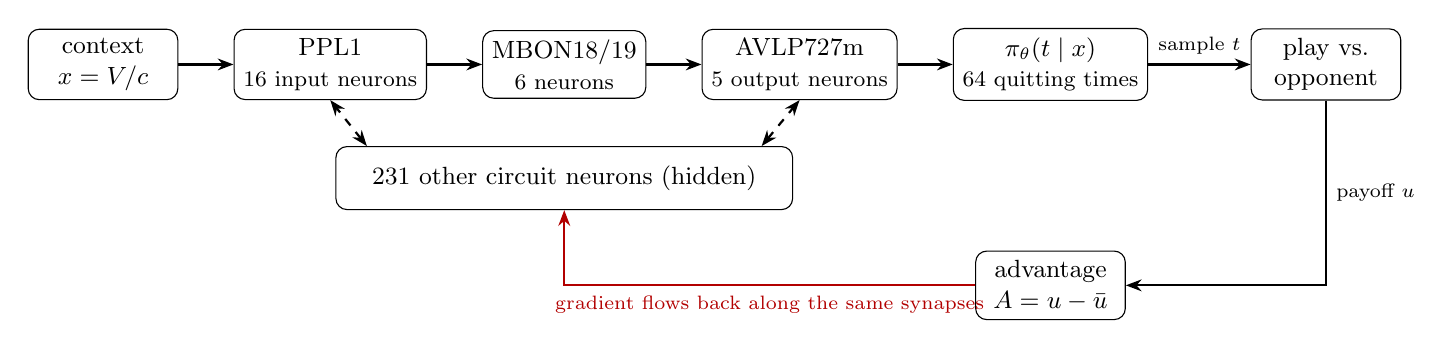
\begin{tikzpicture}[
  node distance=0.7cm,
  box/.style={draw, rounded corners, minimum width=1.9cm, minimum height=0.8cm, align=center, font=\small},
  arr/.style={-{Stealth[length=2mm]}, thick}]
\node[box] (ctx) {context\\$x = V/c$};
\node[box, right=of ctx] (ppl) {PPL1\\ \footnotesize 16 input neurons};
\node[box, right=of ppl] (mbon) {MBON18/19\\ \footnotesize 6 neurons};
\node[box, right=of mbon] (tk) {AVLP727m\\ \footnotesize 5 output neurons};
\node[box, right=of tk] (pi) {$\pi_\theta(t \mid x)$\\ \footnotesize 64 quitting times};
\node[box, below=0.6cm of mbon, minimum width=5.8cm] (hid) {231 other circuit neurons (hidden)};
\node[box, right=1.3cm of pi] (game) {play vs.\\ opponent};
\node[box, below=1.9cm of pi] (adv) {advantage\\$A = u - \bar u$};
\draw[arr] (ctx) -- (ppl);
\draw[arr] (ppl) -- (mbon);
\draw[arr] (mbon) -- (tk);
\draw[arr] (tk) -- (pi);
\draw[arr] (pi) -- node[above, font=\scriptsize]{sample $t$} (game);
\draw[{Stealth[length=2mm]}-{Stealth[length=2mm]}, thick, dashed] (hid.north west) ++(0.4,0) -- (ppl.south);
\draw[{Stealth[length=2mm]}-{Stealth[length=2mm]}, thick, dashed] (hid.north east) ++(-0.4,0) -- (tk.south);
\draw[arr] (game.south) |- node[pos=0.25, right, font=\scriptsize]{payoff $u$} (adv.east);
\draw[arr, red!70!black] (adv.west) -| node[pos=0.25, below, font=\scriptsize, text=red!70!black]{gradient flows back along the same synapses} (hid.south);
\end{tikzpicture}}
\caption{One learning step. The context enters through the PPL1 neurons, spreads through the 258-neuron circuit for 6 steps, and is read out from the AVLP727m neurons as a distribution over quitting times. The agent samples a time, plays, and receives a payoff. The advantage is sent back through the circuit by backpropagation, which follows the fly's wiring in reverse and updates each synapse weight.}
\label{fig:loop}
\end{figure}

\begin{algorithm}[t]
\caption{Sampled self-play with circuit-wired agents}
\label{alg:train}
\begin{algorithmic}[1]
\State Build $\G$ from the connectome; for each of $M$ agents, create weights $\theta^m$ on the edges of $\G$
\For{round $\tau = 1, \dots, T$}
  \State Randomly pair the agents
  \For{each agent $m$}
    \State Run the circuit for $L$ steps on $x$ to get $\pi_{\theta^m}(\cdot \mid x)$ \Comment{Step 2}
    \State Play $B$ matches: sample $t_j \sim \pi_{\theta^m}$, get payoff $u_j$ and outcome $o_j$ \Comment{Step 3}
    \State $A_j \gets \alpha(o_j)\,(u_j - \bar u^m)$;\quad $\bar u^m \gets (1-\beta)\,\bar u^m + \beta \cdot \mathrm{mean}_j(u_j)$
    \State Backpropagate through the unrolled circuit to get $\hat g^m = \frac1B \sum_j A_j \nabla \log \pi_{\theta^m}(t_j \mid x)$ \Comment{Step 4}
    \State Update $\theta^m$ with Adam (or take 4 PPO steps on $L^{\mathrm{clip}}$)
  \EndFor
  \State Every 25 rounds: compute exact exploitability of each agent against the others
\EndFor
\end{algorithmic}
\end{algorithm}

\subsection{A note on biological realism}

Backpropagation is not how a real fly learns. We use it because it is the standard way to train a network, and our question is about the wiring as a learning substrate, not about the fly's own learning rule. In the fly, PPL1 dopamine is thought to act as a teaching signal. We feed the context into PPL1 as an input, which is a modelling choice we keep fixed across all networks so the comparison stays fair.

% ==================================================================
\section{Proposed Solutions}
\label{sec:solutions}

\subsection{What we will compare}

We will train the following agents, all with close to the same number of trainable parameters (within $5\%$):
\begin{itemize}
  \item an oracle that plays the known grid equilibrium, used as a reference;
  \item a tabular policy (one learnable score per quitting time), as a sanity check;
  \item a dense two-layer network;
  \item the real circuit, a degree-preserving rewire and a random sparse graph, each with and without sign constraints;
  \item the frozen-synapse version of the real circuit and of its two controls.
\end{itemize}
Each is trained with exact self-play and with sampled self-play (REINFORCE and PPO), and in sampled mode with loss weighting $\rho \in \{1,2,4,8\}$.

\subsection{Metrics}

\begin{itemize}
  \item Exploitability $\expl$, computed exactly on the grid with no sampling. In sampled mode, each agent is measured against the mix of the other agents. This is the main metric.
  \item Time to threshold $\tau_\varepsilon$: the first round at which $\expl \le \varepsilon$, with runs that never get there marked as censored.
  \item Distance of the learned quitting-time distribution from the equilibrium, using total variation and the Wasserstein-1 distance.
  \item The learned survival curve $P(T > t)$, compared with $e^{-t}$ (and with the shifted equilibrium when $\rho > 1$).
  \item Stability: how much the policy still moves in the last $10\%$ of training.
  \item A loser effect: how much an agent's next quitting time drops after a round with many losses, which is what real defeated flies show.
\end{itemize}

\subsection{Results we plan to show}

\begin{itemize}
  \item Learning curves of exploitability over training for every agent, in both modes.
  \item A table of final exploitability and time to threshold for every agent, with confidence intervals.
  \item The main comparison: real circuit versus rewire versus random graph, with the differences $\delta_{\mathrm{rew}}$ and $\delta_{\mathrm{rand}}$ and whether they are significant.
  \item The learned survival curves against the exponential equilibrium.
  \item The effect of sign constraints, and of trained versus frozen synapses.
  \item REINFORCE versus PPO, to see whether a more stable learning rule changes the picture.
  \item Final exploitability as a function of $\rho$, compared with the predicted shifted equilibrium, and whether the wiring changes the loser effect.
\end{itemize}

\subsection{How we will do it}

We will run 20 random seeds per setting in exact mode and 10 in sampled mode. Learning rates will be tuned per agent on separate seeds, and all circuit-based agents will also be run at one shared learning rate, so that the only difference between them is the wiring. For every comparison we will report the mean with a $95\%$ bootstrap confidence interval, an effect size, and a permutation test with Holm correction for multiple comparisons \citep{holm1979}. We will call a difference real only if its interval excludes zero and the corrected $p$-value is below $0.05$. Every circuit will be rebuilt from the raw MaleCNS files and checked against a stored checksum, so the results are reproducible.

As future scope, the same setup extends to a version of the game where each fly privately knows how much it values the prize, which forces the circuit to turn its input into a value-dependent quitting time.

% ==================================================================
\section{Contribution}
\label{sec:contrib}

\begin{table}[h]
\centering
\begin{tabular}{lp{11.5cm}}
\toprule
Member & Tasks \\
\midrule
Suhani & Problem design; extracting the give-up circuit from the MaleCNS connectome and building the rewired and random controls; designing the circuit-wired and frozen-synapse policy networks; the training, evaluation and statistics pipeline; running the experiments. \\
\addlinespace
Mayank Choudhary & Mathematical analysis of the game: the exponential equilibrium, the grid equilibrium and its stability, and the shifted equilibrium under loss-weighted learning; the reinforcement learning formulation (exact self-play, REINFORCE, PPO) and the exploitability metric. \\
\addlinespace
Krina Paghadar & Wrote the Preliminaries section; worked with Mayank on the mathematical formulation of the problem. \\
\addlinespace
Nakshatra Lad & Literature survey on the war of attrition and connectome-based learning; drafting the Introduction; figures and report formatting. \\
\bottomrule
\end{tabular}
\end{table}

\bibliographystyle{unsrtnat}
\bibliography{references}

\end{document}
